\subsection{Excercise CarRentalStructs}
\label{sec:car_rental_structs}
This task introduces the concept of structs and arrays in go.
The goal is to apply the described concept described in the tasks above to the given code.

By creating structs and arrays a general understanding of the concept of storing and accessing data is developed.

\subsubsection*{Add the Attributes to Structs}
According to \cite{W3S-STR}, a struct creates a collection of members of different types into a single object.
The difference to arrays is that the members can be of different types.

A struct can be defined by using the keyword \texttt{type} followed by the name of the struct and the keyword \texttt{struct}.
Then the attributes and their datatypes are defined within curly brackets.
Struct members can be accessed by using the dot operator after the struct name.

Structs can be used to store data in a structured way.
It can also be used for passing and returning multiple values from a function.

The goal of this task is to add the attributes from the entities Car and Rental as specified in \autoref{fig:extendedEntityDiagram} to the structs.

After adding the attributes from the entity diagram to the \hfill \newline \texttt{.../golang/CarRental/CarRentalStructs/CarRentalStructs.go} path and saving
the IDE automatically formats the code and indents it correctly.

The code is specified in \autoref{lst:car_rental_structs}.
\begin{lstlisting}[
style=kit-cm,
language=Golang,
caption={Structs of CarRentalStructs.go after adding the Attributes from the Entity Diagram},
label={lst:car_rental_structs}
]
\\ CarRentalStructs.go
\\ Author: Felix Weik

type Customer struct {
	id         int
	Name       string
	rentals    []Rental
}

type Rental struct {
	id          int
	startDate   Date
    endDate     Date
}

type Car struct {
	id          int
	carType     string
}

type Date struct {
	day         int 
    month       int 
    year        int 
}
\end{lstlisting}

\subsubsection*{Initialize and Print Structs}
Structs are organized in key-value pairs.
The key is the name of the attribute and the value is the value of the attribute.
By using the dot operator, this data can be accessed.
The key to this task is to initialize the structs and print them to the console.

The code for printing the structs is shown in \autoref{lst:car_rental_print_structs}.
The \texttt{fmt.Printf()} function is used to print the structs.
The \texttt{\%+v} is used to print the structs in a human-readable way.
\texttt{\%v} is a formatting verb used to represent values in a default way.
Adding the \texttt{+} flag the data is displayed in a structured way, which is particularly useful for structured data like structs.
The struct-name after the comma defines the struct that will be printed where the placeholder is located.

The result of the initialization and printing of the structs is shown in \autoref{fig:car_rental_structs}.
\begin{figure}[H]
    \centering
    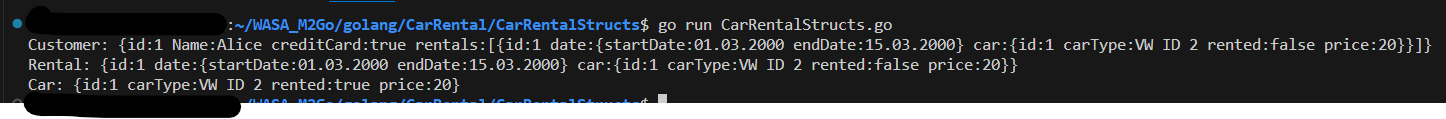
\includegraphics[width=\textwidth]{figures/goLang/carRental/carRental_structs.png}
    \caption{Output of the structs}
    \label{fig:car_rental_structs}
\end{figure}

\begin{lstlisting}[
style=kit-cm,
language=Golang,
caption={Printing the Structs},
label={lst:car_rental_print_structs}
]
// CarRentalStructs.go

fmt.Printf("Customer: %+v\n", customer1)
fmt.Printf("Rental: %+v\n", rental)
fmt.Printf("Car: %+v\n", car)
\end{lstlisting}

\subsubsection*{Create an Array of Rentals}
The function works as follows:
\begin{enumerate}
    \item The array \texttt{cartypes} holds the string of five different car types
    \item The function \texttt{createRentals(id, date, car)} returns five rentals that are appended to the array
    \item Via \texttt{fmt.Println(rentals)} the array is printed into the console
\end{enumerate}

The result is shown in \autoref{fig:car_rental_array_five_rentals}.

The initialization process of an empty array containing five cars in go looks as follows: \texttt{var cars [5]Car}
Alternatively the array can be created already initialized with \texttt{var cartypes = [5]string\{"Type1", ..., "Type5"\}}
This notation creates an array of 5 strings representing cartypes.

A for loop in go ranges from an integer value, usually called "i", to an upper border.
The value will usually be incremented by one until the upper border is reached. 
The code within the loop will be executed until it reaches the upper border.
A correct implementation for five iterations is shown in \autoref{lst:for_loop_init}.

\begin{lstlisting}[
style=kit-cm,
language=Golang,
caption={Initialization of a For-Loop iterating five Times},
label={lst:for_loop_init},
]
for i := 0; i < 5; i++ {
    // Run some code
}
\end{lstlisting}

\begin{figure}[H]
\centering
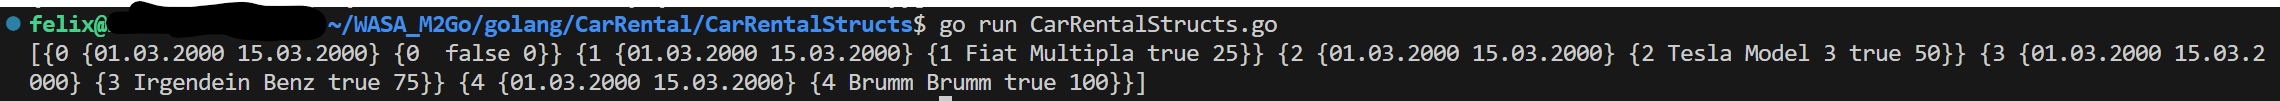
\includegraphics[width=\textwidth]{figures/goLang/carRental/carRental_arrayFiveRentals.png}
\caption{Output of the Array of Rentals}
\label{fig:car_rental_array_five_rentals}
\end{figure}

\subsection{Excercise CarRentalTests}
\label{sec:car_rental_tests}
This task introduces the concept of testing in Go.
It also introduces the Open-Constraint-Language (OCL) and how to implement it in Go.

A listing is given containing the OCL constraints.
The goal of this task is to analyze these constraints, check their implementation in go, run the tests and add additional test cases.

\subsubsection*{Analyze OCL Constraints}
In the given task four invariants are described.
These invariants stand under the context of the date object.
Therefore the invariants are implemented in the date object.

These invariants are implemented in \texttt{./CarRentalTests/CarRentalTests.go} \hfill \linebreak and executed in \texttt{./CarRentalStructs/CarRentalStructs.go}.

The first invariant checks if the year is greater than or equal to 2000.
The second invariant checks if the month is less than 13.
The third invariant checks if the month is greater than or equal to 1.
The fourth invariant checks if the number of days in the month is valid.

The following enumeration depicts the lines of code where the invariants are implemented.
\begin{enumerate}
    \item \texttt{self.Date.Year >= 2000}: CarRentalTests.go line 20-22
    \item \texttt{self.Date.Month < 13}: CarRentalTests.go line 24-26
    \item \texttt{self.Date.Moth >= 1}: CarRentalTests.go line 24-26
    \item \texttt{self.ValidateNumberOfDaysInMonth() == True}: CarRentalTests.go line 32
\end{enumerate}

\subsubsection*{Run Test}
After running the test function an error occurs. 
The test, therefore, does not pass.
The error is shown in \autoref{fig:car_rental_test_error}.

This error is caused due to a false implementation in line 20 of \hfill \linebreak \texttt{./CarRentalTests/CarRentalTests.go}
In the first test, it checks if the year is greater than 2000, yet for correct execution, it needs to be greater than or equal to 2000.

\begin{figure}[H]
    \centering
    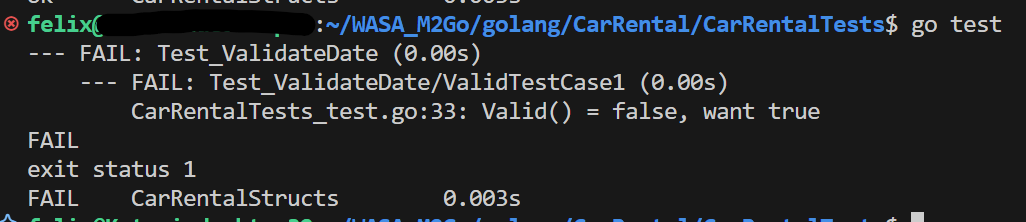
\includegraphics[width=0.8\textwidth]{figures/goLang/carRental/carRental_dateTestError.png}
    \caption{Error of the Test}
    \label{fig:car_rental_test_error}
\end{figure}

\subsubsection*{Correct Code}
As mentioned in the subsection above, line 20 is not implemented correctly.
By changing line 20 from \texttt{if !(d.Year \> 2000)} to \texttt{if !(d.Year \>\= 2000)} the code will execute correctly and the test passes.
The working tree of the changes is shown in \autoref{fig:car_rental_test_working_tree}.

\begin{figure}[H]
    \centering
    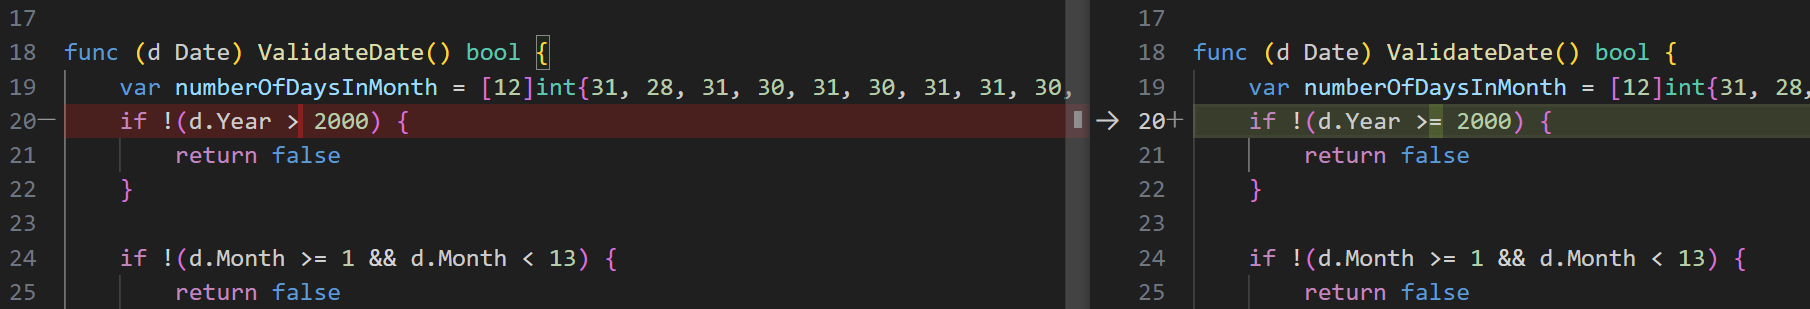
\includegraphics[width=\textwidth]{figures/goLang/carRental/carRental_dateTestWorkingTree.png}
    \caption{Working Tree of the Changes}
    \label{fig:car_rental_test_working_tree}
\end{figure}

\subsubsection*{Invalid Test Case}
Implementing an invalid test case the following code is added to the test function:
\begin{lstlisting}[
style=kit-cm,
language=Golang,
caption={Invalid Test Case},
label={lst:invalid_test_case}
]
name:   "InvalidTestCase1",
fields: fields{Day: 12, Month: 13, Year: 2000},
want:   false,  
\end{lstlisting}

As shown in \autoref{lst:invalid_test_case} the month is set to 13, which is invalid.
Therefore the test should return false.
The test, however, runs successfully due to the want value set to false.
